\documentclass[11pt]{article}
\usepackage[a4paper,margin=2.35cm]{geometry}
\usepackage{amsmath,amssymb,amsthm,booktabs,graphicx,float,array,microtype}
\usepackage[colorlinks=true,allcolors=blue]{hyperref}
\usepackage[font=small,labelfont=bf]{caption}
\usepackage{enumitem}
\graphicspath{{figures/}}
\newtheorem{proposition}{Proposition}
\newtheorem{theorem}{Theorem}
\newtheorem{corollary}{Corollary}
\newcommand{\nrmse}{\operatorname{NRMSE}}
\newcommand{\indet}{\textsc{Unresolved}}
\title{Identifiability-Aware Selection of Shared Finite-Memory Models\\from Sparse Multichannel Relaxation Data}
\author{Haitao Duan$^{1}$, Ning Hu$^{2,*}$, Shuqun Li$^{3}$, Chuyang Hu$^{4}$\\[2mm]
\small $^1$School of Computer Science, Hangzhou Dianzi University, Hangzhou, China\\
\small $^2$School of Mechanical Engineering, Hangzhou Dianzi University, Hangzhou, China\\
\small $^3$School of Mathematics and Physics, Xi'an Jiaotong-Liverpool University, Suzhou, China\\
\small $^4$Department of Computer Science and Engineering,\\
\small University of California, Santa Cruz, CA 95064, USA\\[1mm]
\small $^*$Corresponding author: \href{mailto:huning@hdu.edu.cn}{huning@hdu.edu.cn}}
\date{}

\begin{document}
\maketitle

\begin{abstract}
Finite exponential models are routinely used to report relaxation timescales, yet a lower residual does not show that an additional timescale is resolved by the experiment. An identifiability-aware selection method is developed for sparse multichannel relaxation data. Decay rates are shared across independent specimens or material groups, while amplitudes and offsets remain unit specific. A candidate order is retained only when information gain, held-unit early-to-late prediction, foldwise rate stability, and adjacent-rate resolution agree; otherwise the data are reported as insufficient to resolve the order. Rate coalescence limits this inference because adjacent exponential sensitivities become nearly collinear on a finite noisy window. A Gaussian two-point bound describes this limitation and motivates a design-conditional diagnostic. Across four residual generators, all 160 separated rank-two trials were retained and all 160 coalesced trials remained unresolved. On public PVA relaxation data, only the complete 28-s, 96-sample design supports a three-rate realization; its held-specimen median NRMSE decreases from 0.01757 at rank one to 0.00932 at rank three. For 17 copper-alloy tests in nine material groups, ordinary BIC favors rank three, whereas an AR(1)-profile criterion and held-group prediction support rank one; rank-three held-group NRMSE reaches 104.25. Gas-sensor and hydraulic data serve as scope tests: predictive or in-sample gains do not justify an order when rates coalesce or fail to transfer. These results relate observation design to the finite-memory interpretation supported by grouped data and retain insufficient resolution as a possible outcome.
\end{abstract}

\noindent\textbf{Keywords:} relaxation modelling; finite memory realization; identifiability; model-order selection; observation design; correlated residuals

\section{Introduction}
Hereditary systems are often compressed into finite sums of exponentials. The fitted poles are then interpreted as relaxation times, auxiliary states, or reduced memory modes. This practice is useful in materials characterization and reduced modelling, but it creates a recurrent inference problem: finite windows, correlated residuals, and repeated channels can make several fitted poles appear stable even when the experiment cannot resolve them. Classical Prony recovery and vector fitting provide effective reconstruction machinery \cite{stampfer2020gop,gustavsen1999vector,bosner2021parallel}, while recent generalized Langevin models learn expressive memory kernels from trajectories \cite{lei2016parameterization,ge2024state,lang2026learning}. Neither reconstruction accuracy nor predictive accuracy alone answers the question studied here: what is the smallest shared finite realization supported across independent experimental units?

A decision rule is needed to distinguish representation quality from mechanism resolution. Additional modes can absorb correlated noise, nearby rates generate nearly collinear sensitivity columns, and channels from one experiment do not constitute independent evidence. A model may consequently predict held observations while its internal spectrum remains unresolved. Model order is therefore increased only when the relevant numerical and cross-unit evidence agrees.

Model-order support is assessed at the level of independent specimens or material groups by combining information gain, held-unit transfer, foldwise rate stability, and local rate resolution. An adjacent-rate testing bound and a conditional consistency result for an independently calibrated diagnostic relate unresolved orders to sensitivity coalescence. The resulting decision rule is then expressed as observation-design criteria and examined under alternative residual models on two public material-relaxation datasets. Semi-synthetic controls evaluate its behavior at known rank, while two external dynamic datasets test its response when improved fit does not support a finite-memory interpretation. The calculations and decision records are provided in reproducible form.

The main applications are public PVA and copper-alloy stress-relaxation datasets, which test transfer across physical specimens and material groups \cite{schelkow2026pva,kupferdigital2024relaxation}. A chemically distinct gas-sensor dataset and a hydraulic-system dataset are used as scope tests \cite{uci308gas,ziyatdinov2015dataset,ziyatdinov2015bioinspired,helwig2015hydraulic}. The validation is tiered by purpose: known-rank controls evaluate the decision rule, material data examine its intended use, and the external tasks identify cases in which improved fit or prediction does not support a mechanistic order.

\section{Relation to existing methods}
Finite exponential and rational representations have a long numerical history. Generalized Prony methods recover sparse eigenfunction expansions and analyze reconstruction sensitivity \cite{stampfer2020gop}; matrix-pencil variants extend recovery to multivariate observations \cite{bosner2021parallel}; and vector fitting estimates shared poles from frequency-domain responses \cite{gustavsen1999vector}. These methods provide the representation and baseline machinery used here. The analysis addresses evidential support for a shared order under noisy grouped observations; no new reconstruction solver is introduced.

In data-driven non-Markovian modeling, rational auxiliary-state parameterizations and learned memory kernels support accurate reduced dynamics \cite{lei2016parameterization,ge2024state,lang2026learning}. Their primary objective is kernel estimation or dynamical prediction. The question considered here is instead the minimum finite realization supported across independent units, with no order assigned when the observations cannot separate candidate mechanisms.

Relaxation-spectrum identification is also established in viscoelasticity, where regularization and time-scale selection stabilize inverse recovery \cite{stankiewicz2023relaxation}. Closely spaced exponential nodes are intrinsically ill-conditioned through their Vandermonde geometry \cite{moitra2015superresolution}; this motivates leaving order unresolved rather than forcing selection. Classical BIC and small-sample time-series corrections further show why parameter count and residual dependence must be separated \cite{schwarz1978bic,hurvich1989timeseries}. In the present method, these estimators are evaluated together with held-unit prediction, foldwise rate stability, and rate separation. No individual criterion is treated as sufficient.
Classical model-order research distinguishes information-criterion evidence, predictive selection, and Bayesian evidence rather than treating them as equivalent \cite{stoica2004modelorder,shao1993crossvalidation,kass1995bayes}. Selective prediction likewise formalizes abstention when a requested risk cannot be supported \cite{geifman2017selective}. Here, an unresolved result refers to a shared dynamical-rank interpretation rather than an individual class prediction. The four criteria specialize this general principle to grouped relaxation data.

\section{Model and identifiability-aware selection method}
\subsection{Shared finite realization}
For experimental unit $i$ observed at times $t_{ij}$, the candidate rank-$r$ model is
\begin{equation}
y_i(t)=c_i+\sum_{k=1}^{r}a_{ik}\exp(-\lambda_k t)+\varepsilon_i(t),
\qquad a_{ik}\in\mathbb R,\quad 0<\lambda_1<\cdots<\lambda_r.
\label{eq:model}
\end{equation}
The rates $\lambda_k$ are shared across units; amplitudes $a_{ik}$ and offsets $c_i$ are unit specific. This factorization separates a candidate common spectrum from experimental scale and baseline differences. It is appropriate only on a declared interval where positive finite exponential relaxation is a plausible representation.
If $t$ is measured in a declared time unit $T$, then $\lambda_k$, $\gamma_j$, and $\omega_j$ below have units $T^{-1}$; amplitudes, offsets, observations, and residuals have the response unit. Every logarithm of a rate is taken relative to a fixed reference rate $\lambda_{\mathrm{ref}}$.

\subsection{Four selection criteria}
Candidate ranks $r=1,\ldots,r_{\max}$ are fitted using training units. The smallest rank is supported only if it satisfies all four criteria.

\paragraph{Information criterion.} Let $n$ be the number of fitted observations and $q_r$ the number of free parameters. The independent-residual score is
\begin{equation}
\mathrm{BIC}_r=n\log\!\left(\frac{\mathrm{SSE}_r}{n s_y^2}\right)+q_r\log n,
\end{equation}
where $s_y>0$ is a fixed response scale declared before rank comparison. A candidate rank must improve this score over the lower rank by a predeclared margin \cite{schwarz1978bic}. All reported tasks use dimensionless registered responses and $s_y=1$, so this normalization leaves the recorded BIC values unchanged. Because relaxation residuals are serially correlated, every final audit additionally reports a Gaussian AR(1) profile-BIC and an effective sample-size diagnostic. Agreement is supporting evidence; disagreement triggers sensitivity reporting rather than retrospective threshold selection \cite{hurvich1989timeseries}.


\paragraph{Transfer criterion.} Complete experimental units are held out. Rates are learned from the remaining units, amplitudes are calibrated on the first 60\% of the held curve, and the final 40\% is predicted. Error is summarized by
\begin{equation}
\nrmse_i=\frac{\|\hat{\mathbf y}_{i,\mathrm{late}}-\mathbf y_{i,\mathrm{late}}\|_2}
{\|\mathbf y_{i,\mathrm{late}}-\bar y_{i,\mathrm{late}}\mathbf 1\|_2+\epsilon}.
\end{equation}
$\epsilon>0$ has the same units as the response norm and only prevents division by zero; after registered normalization, $\epsilon=10^{-12}$ is used.

\paragraph{Stability criterion.} Foldwise log-rates must remain sufficiently stable. For each mode, the standard deviation of $\log(\lambda_k/\lambda_{\mathrm{ref}})$ across held-unit folds must not exceed a predeclared tolerance.

\paragraph{Separation criterion.} Adjacent rates must satisfy
\begin{equation}
\min_k\frac{\lambda_{k+1}}{\lambda_k}\ge \rho_{\min}>1.
\label{eq:separation}
\end{equation}
This prevents a numerically improved but coalesced spectrum from being interpreted as distinct timescales.

If no rank satisfies all criteria, the model order is \indet{}. This is not an optimization failure: it records that the declared observations do not support the requested mechanism-level resolution.

\begin{figure}[H]
\centering
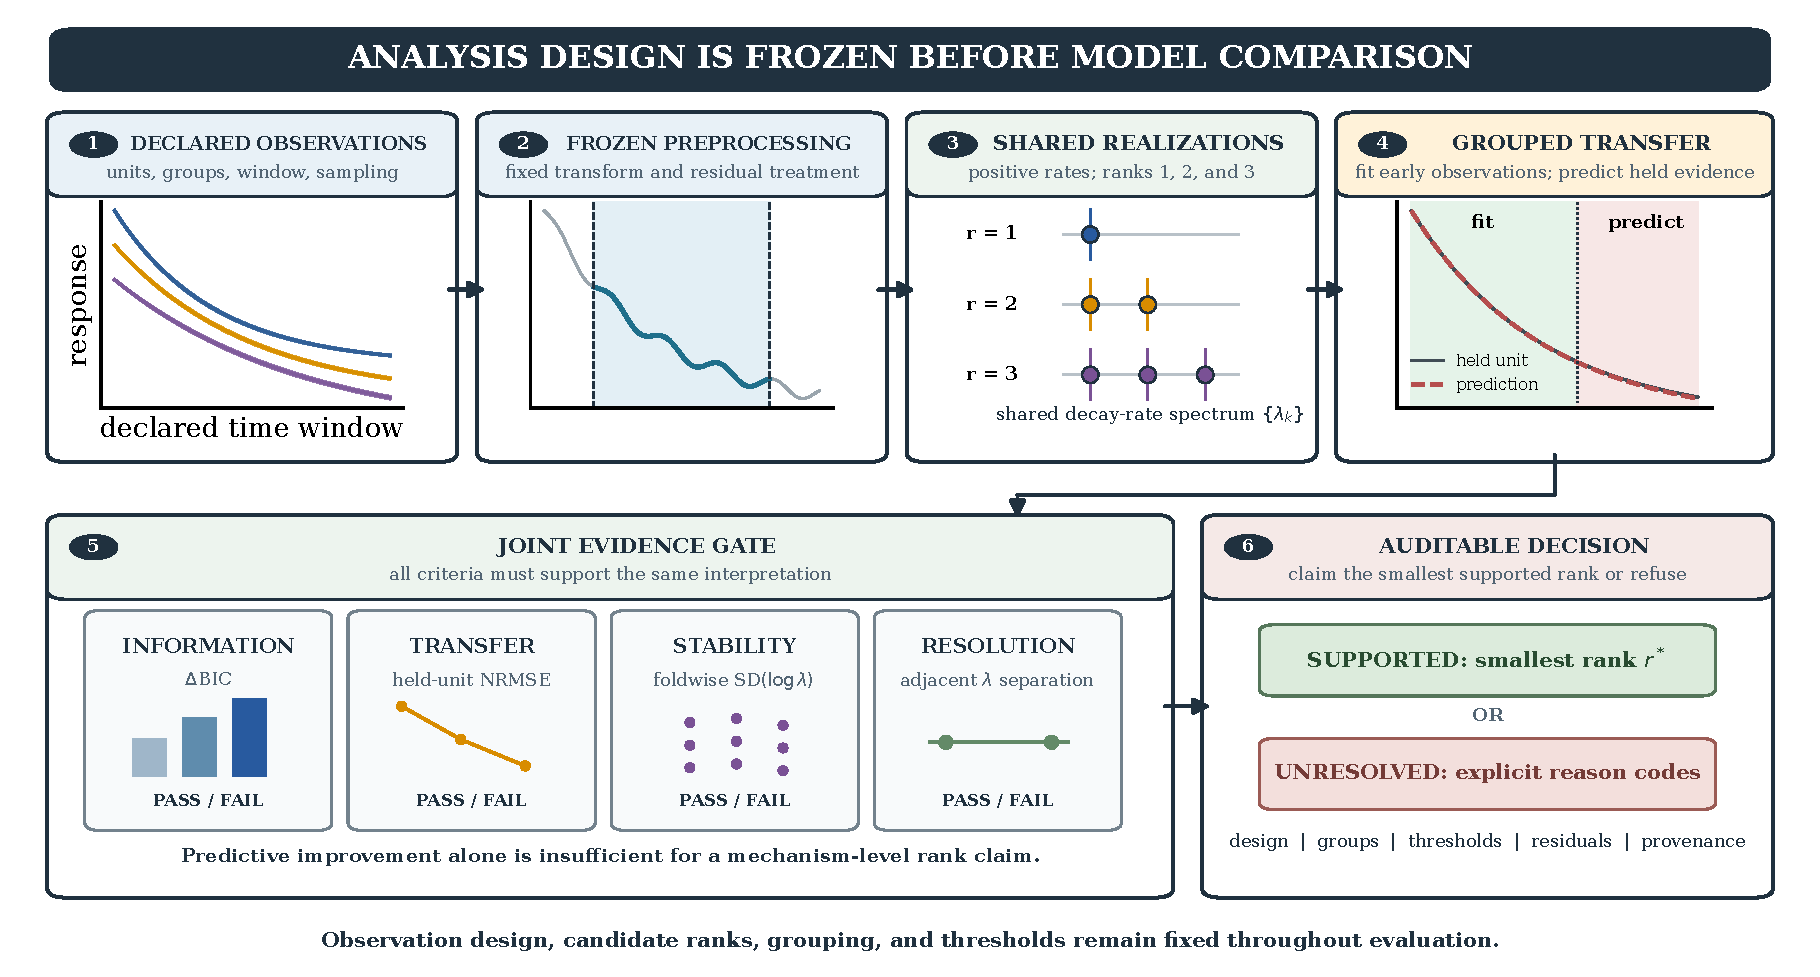
\includegraphics[width=0.96\textwidth]{fig_stage62_method_workflow.pdf}
\caption{\textbf{Frozen grouped model-selection workflow.} Observation design, grouping, residual treatment, candidate ranks, and thresholds are declared before fitting. Shared-rate realizations are evaluated by held-unit transfer together with information gain, foldwise rate stability, and adjacent-rate resolution. The output is the smallest supported rank; when no rank satisfies all criteria, the unresolved result is recorded with its diagnostic basis and provenance. Curves and gate glyphs are schematic; quantitative evidence is reported in the subsequent figures and tables.}
\label{fig:workflow}
\end{figure}

\subsection{Minimal identifiability analysis}
Let $\boldsymbol\mu(\theta)$ stack the mean responses and let $J=\partial\boldsymbol\mu/\partial\theta$. Rate coordinates are $\vartheta_k=\log(\lambda_k/\lambda_{\mathrm{ref}})$. Local identification requires that the corresponding columns remain linearly independent after nuisance amplitudes and offsets are projected out.

\begin{proposition}[Local rate identification]
If the projected rate-sensitivity matrix $J_\lambda$ has full column rank at $\theta^\star$, then the shared rates are locally identifiable in a neighborhood of $\theta^\star$. If its smallest singular value tends to zero, local uncertainty diverges and distinct nearby rates cannot be stably resolved.
\end{proposition}
\begin{proof}
Full column rank makes the local Fisher/Gauss--Newton matrix $J_\lambda^\top WJ_\lambda$ positive definite for positive definite $W$. The inverse-function argument gives local injectivity. Vanishing smallest singular value makes the inverse sensitivity unbounded.
\end{proof}

For two close rates $\lambda$ and $\lambda+\delta$, the mean-value theorem gives
\begin{equation}
|e^{-\lambda t}-e^{-(\lambda+\delta)t}|
\le |\delta|t e^{-\min(\lambda,\lambda+\delta)t}.
\label{eq:coalescence}
\end{equation}
Thus a finite noisy window may not distinguish the pair even when the two-mode fit lowers residual error. Equation~\eqref{eq:coalescence} motivates the separation criterion, while the singular spectrum of $J_\lambda$ supplies a continuous diagnostic.

Raw sample count alone is not an information measure. Under correlated residuals with covariance $\Sigma$, local information is $J^\top\Sigma^{-1}J$. Extending the horizon changes the sensitivity geometry and residual correlation simultaneously; denser sampling can add nearly redundant rows. Support boundaries therefore need not be monotone in sample count.

The adjacent-rate limit can be stated formally. Consider independent Gaussian observations with variance $\sigma^2$ and an alternative containing $a_i e^{-\lambda t}+b_i e^{-(\lambda+\delta_n)t}$. Its merged lower-rank comparison uses $(a_i+b_i)e^{-\lambda t}$. Define
\begin{equation}
R_n^2=\frac{\delta_n^2}{\sigma^2}\sum_{i,\ell}b_i^2t_{i\ell}^2
e^{-2\min(\lambda,\lambda+\delta_n)t_{i\ell}}.
\label{eq:boundary-index}
\end{equation}

\begin{theorem}[Gaussian adjacent-rate indistinguishability]
Under the declared Gaussian model, $\mathrm{KL}(P_{r,n}\|P_{r-1,n})\le R_n^2/2$. If $R_n\to0$, every measurable rank test obeys $\alpha_n+\beta_n\to1$; hence no uniformly consistent rank decision exists along this sequence.
\end{theorem}
\begin{proof}
The mean difference is $d_{i\ell}=b_i[e^{-(\lambda+\delta_n)t_{i\ell}}-e^{-\lambda t_{i\ell}}]$. Equation~\eqref{eq:coalescence} bounds $\|d\|_2^2/\sigma^2$ by $R_n^2$. The common-covariance Gaussian formula gives the KL bound. Pinsker's inequality and the two-point testing bound yield $\alpha_n+\beta_n\ge1-\operatorname{TV}(P_{r,n},P_{r-1,n})\ge1-R_n/2$ \cite{tsybakov2009nonparametric}.
\end{proof}

\begin{corollary}[Embedded multi-rate obstruction]
Suppose all nuisance components and all rates except one adjacent pair are fixed or estimated with error $o(R_n)$. The rank-$r$ and merged rank-$(r-1)$ classes then contain the two-point subexperiment of the theorem. Consequently, if $R_n\to0$, no test can be uniformly consistent over the larger classes.
\end{corollary}
\begin{proof}
Restrict the larger parameter spaces to the two distributions used in the theorem. Uniform consistency on the larger spaces would imply consistency on this restricted pair, contradicting the theorem.
\end{proof}
\begin{corollary}[Conditional consistency of a calibrated resolution criterion]
Let $\widehat R_n$ satisfy $|\widehat R_n-R_n|=o_p(c_n)$ on a fixed observation-design sequence, where $c_n\downarrow0$ is calibrated independently of the evaluation sample. If $R_n=o(c_n)$, then the rule $\widehat R_n\le c_n$ leaves the order unresolved with probability tending to one. Under fixed adjacent-rate separation, diverging minimum projected information eigenvalue, consistent parameter estimation, and consistent remaining criteria, the rule accepts the true rank with probability tending to one.
\end{corollary}

These results are local or embedded statements. They do not establish global identifiability for unrestricted nonlinear kernels, irregular designs, non-Gaussian noise, or jointly drifting nuisance parameters. The implementation reports a local proxy $\widehat D$: sensitivities with respect to $\log(\lambda_k/\lambda_{\mathrm{ref}})$ are projected off curve-specific offset and amplitude columns, and the smallest projected singular value is multiplied by the minimum adjacent log-rate gap and divided by residual noise. Division by the square root of the observation count removes its leading sample-size scaling. The implemented proxy is not asserted to estimate $R_n$ without additional assumptions. It is calibrated on a declared semi-synthetic design and evaluated on disjoint seeds, and remains a task-internal diagnostic rather than a universal threshold.

\subsection{Declared extensions beyond positive fully shared rates}
Four scoped extensions are tested without changing the frozen decisions on the four public datasets. Stable oscillatory memory is represented by real conjugate-pole blocks,
\begin{equation}
y_i(t)=c_i+\sum_k a_{ik}e^{-\lambda_k t}+\sum_j e^{-\gamma_j t}\{u_{ij}\cos(\omega_jt)+v_{ij}\sin(\omega_jt)\}+\varepsilon_i(t),
\label{eq:oscillatory-extension}
\end{equation}
where $\gamma_j,\omega_j>0$. Each extension targets one assumption of Eq.~\eqref{eq:model}: conjugate poles test the positive-real-pole restriction; partial sharing uses $\log(\lambda_{gk}/\lambda_{\mathrm{ref}})=\mu_k+\delta_{gk}$ with $\sum_g\delta_{gk}=0$ to test exact sharing; a dense log-normal relaxation measure tests the finite-spectrum assumption; and a group-level conformal audit tests exchangeable group calibration. Partial sharing uses a declared penalty $\eta\sum_{g,k}\delta_{gk}^2$, selected without the final evidence group. For $m$ exchangeable calibration groups, the conformal upper threshold is the $\lceil(m+1)(1-\alpha)\rceil$-th order statistic (capped at $m$), and the upper-tail test value is $(1+\#\{S_j\ge S_{\rm test}\})/(m+1)$ \cite{shafer2008conformal}. This is a finite-sample marginal statement under group exchangeability, not a guarantee after group shift.
\section{Numerical design and material-relaxation applications}
\subsection{PVA stress relaxation}
The first task uses the public stress-relaxation dataset of cylindrical PVA gel polymer electrolyte samples \cite{schelkow2026pva}. It contains three specimens and three cycles per specimen. No smoothing is applied. Rates are learned with leave-one-specimen-out folds, and the complete 28-s task contains 96 retained points per curve. Because only three specimens are independent, curve-level uncertainty summaries are descriptive and are not treated as population-level inference.

\subsection{Copper-alloy stress relaxation}
The second task uses the public KupferDigital mechanical-testing archive \cite{kupferdigital2024relaxation}. Seventeen physical stress-relaxation test files from nine material-code groups are treated as independent experimental units. Engineering stress is divided by the first registered stress, and each curve is registered without smoothing on a common 96-point grid from zero to the shortest complete endpoint within the declared 24-hour tests. Complete material-code groups are held out, so repeated specimens from one group never cross a fold. The decision concerns a shared empirical relaxation realization and is not evidence for a unique microscopic mechanism.

\subsection{Gas-sensor recovery}
The third task uses UCI dataset 308 \cite{ziyatdinov2015dataset}. Fifty non-air exposure experiments are retained from five acquisition batches. Each experiment contains 16 metal-oxide sensor channels. The analysis is restricted to the registered 180--300 s recovery interval, summarized by medians over the physical 12-s modulation cycle. Channels remain clustered within an exposure, and complete acquisition batches are held out. Thresholds and the 60/40 calibration/prediction split are frozen before fitting.

\subsection{Hydraulic cooling transients}
The fourth task uses UCI dataset 447, acquired from a hydraulic test rig over repeated 60-s load cycles \cite{helwig2015hydraulic}. It is an external multichannel dynamic stress test selected for repeated controlled states and clustered sensors; it is not presented as validation of a component-level relaxation mechanism. Valve condition, pump leakage, accumulator pressure, and the stability flag are fixed; cooler efficiency varies over 3\%, 20\%, and 100\%. Ten independent cycles are retained per state. Four channels (cooling efficiency, cooling power, and two temperatures) are analyzed over seconds 20--55 without smoothing. Normalization uses only the first 22 samples of the declared window. Complete cooler states are held out, and channels remain clustered within their cycle.

\subsection{Baselines and statistical audits}
The gas task compares the shared-rate model with independent nonlinear rank-three fitting, fixed-grid nonnegative least squares (NNLS), and a Prony recurrence baseline. The hydraulic task adds stretched-exponential, AR(2), Prony, and fixed-grid NNLS early-to-late controls. Copper-alloy ranks are compared by leave-one-material-group-out prediction, ordinary BIC, and an AR(1)-profile BIC sensitivity analysis. All methods use identical task-specific splits. Paired comparisons use independent exposure experiments, cycles, specimens, or test files rather than within-unit channels or repeated samples. Robustness checks include clustered bootstrap intervals, one-sided paired Wilcoxon tests, 1/2/4/8 optimizer starts, leave-one-group-out transfer, and a $3\times3\times3$ threshold grid. Baseline $p$-values are Holm adjusted separately within each public-task comparison family to control family-wise error. Threshold scans audit sensitivity; they are not used to choose thresholds after observing outcomes.

\section{Results}
\subsection{Evidence hierarchy}
The evidence has three distinct levels. Semi-synthetic controls have known generating rank and evaluate decision behavior under the declared noise processes. Public tasks assess finite empirical realization, transfer, stability, and unresolved-order decisions on observed grouped data, but do not supply microscopic rank labels. Mechanistic identification would require independent physical labels or interventions and is outside the present evidence. A supported public-data rank consequently denotes the smallest finite realization satisfying the predeclared criteria, whereas \indet{} denotes insufficient evidence under those criteria.

The figures are organized by evidential role. Figure~\ref{fig:semisynthetic} evaluates the calibrated decision against known rank, and Fig.~\ref{fig:amm-baselines} compares predictive utility under matched observations. Figure~\ref{fig:pva-boundary} relates experimental horizon and sampling budget to the retained realization, while Fig.~\ref{fig:amm-material} examines transfer and residual-model sensitivity in the material setting. Figures~\ref{fig:baselines}--\ref{fig:hydraulic} provide scope tests in which prediction or in-sample fit can improve without supporting an order. Figure~\ref{fig:extensions} examines four assumptions of the main model. Results from these tasks are not used interchangeably.

\subsection{Calibrated support and unresolved-order controls}
Grouped semi-synthetic experiments supply known-rank controls. A geometric midpoint calibrated on a disjoint split fixes the normalized local-boundary threshold at 0.49085. Without retuning, the rule was evaluated under IID Gaussian, AR(1), AR(2), and heteroscedastic noise. For each generator it accepted all 40 well-separated rank-two trials with true rates $(0.12,0.72)$ and left all 40 coalesced trials with true rates $(0.34,0.37)$ unresolved. Thus each observed rate is 1.00 and its two-sided Wilson 95\% interval is $[0.9124,1]$. These trials quantify transfer across the four declared generators; they are design-conditional evidence, not a universal error guarantee or coverage statement for arbitrary residual processes.

\begin{figure}[H]
\centering
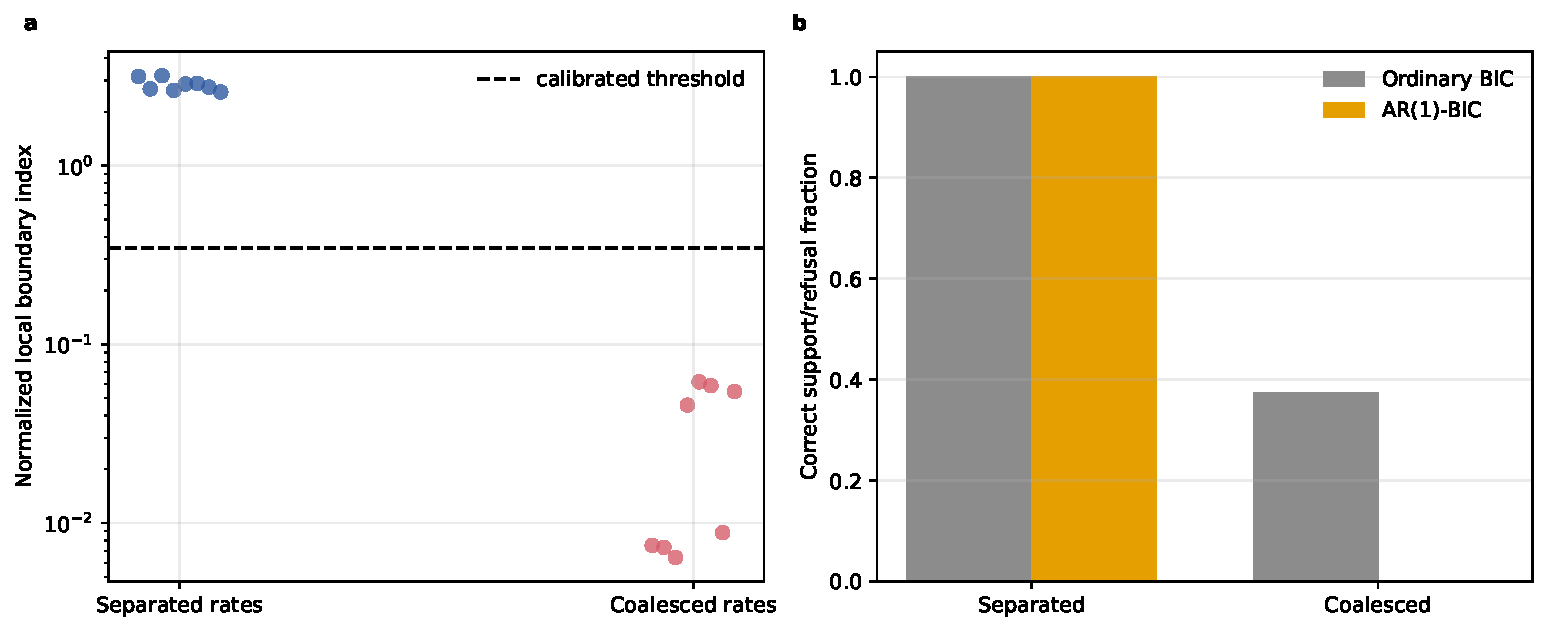
\includegraphics[width=0.90\textwidth]{fig_stage65_acceptance_calibration.pdf}
\caption{Semi-synthetic calibration with disjoint calibration and evaluation seeds. (a) The normalized local-boundary proxy separates the declared well-separated and coalesced designs. (b) Correct support or unresolved-order decisions under ordinary and AR(1)-profile BIC; the explicit resolution criterion is needed because information criteria alone often merge unresolved nearby rates.}
\label{fig:semisynthetic}
\end{figure}

For comparison with direct trajectory alternatives on identical sparse early-time observations, the analysis also includes a regularized damped-modal fit and a trajectory MLP. These baselines are not assigned a memory rank. The shared positive-real realization has the lowest held-horizon error in all three separated-rank controls (Fig.~\ref{fig:amm-baselines}). This result is limited to the declared relaxation family and does not imply general superiority over modal or neural predictors.

\begin{figure}[H]
\centering
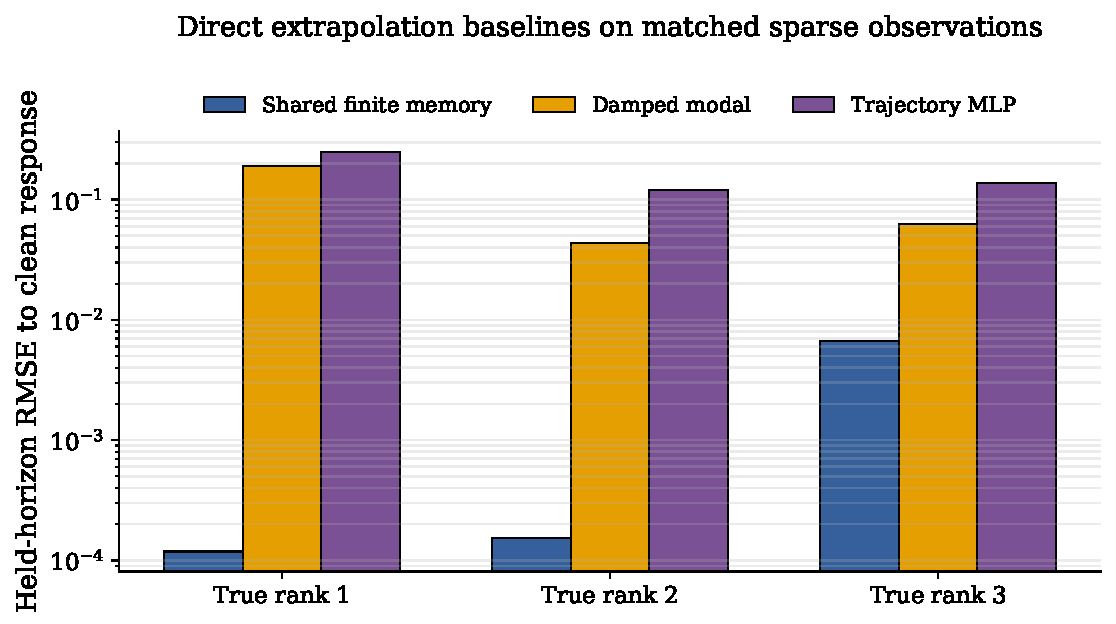
\includegraphics[width=0.82\textwidth]{fig_amm_direct_baselines.pdf}
\caption{Held-horizon extrapolation on matched sparse observations. All methods use the same early-time samples. The damped-modal and MLP baselines are trajectory predictors and their internal dimensions are not interpreted as relaxation rank.}
\label{fig:amm-baselines}
\end{figure}

\subsection{Leave-one-criterion-out decision analysis}
A fixed-record ablation was performed without refitting. PVA boundary records supplied transitions that failed only transfer or only stability; the UCI gas record supplied a transition that failed only separation; and a controlled transition with negative information gain but all other checks passing examined the information criterion. Under the complete rule, each record remained unresolved or stayed at the lower rank. Omitting the single failed criterion promoted the higher rank in all four cases. The criteria are therefore nonredundant on these selected stress records. This logical relevance analysis is not an estimate of population-level variable importance.
\subsection{Independent PVA support and its boundary}
On the complete 28-s task, the selection rule supports rank three. Table~\ref{tab:pva} shows that rank three has the lowest BIC and held-curve NRMSE while satisfying the rate-stability and separation criteria.

\begin{table}[H]
\centering
\caption{PVA public-data result under the predeclared selection rule.}
\label{tab:pva}
\begin{tabular}{rrrr}
\toprule
Rank & Mean BIC & Median held NRMSE & Max. fold log-rate SD\\
\midrule
1 & $-6944.806$ & 0.01757 & 0.0284\\
2 & $-8350.562$ & 0.01121 & 0.1540\\
3 & $-8670.737$ & 0.00932 & 0.3685\\
\bottomrule
\end{tabular}
\end{table}

Rank three improves the median curve error over rank one by 48.4\%, with a descriptive bootstrap interval of [39.5\%, 79.8\%]. The horizon-by-budget map is nonmonotone. At fixed spacing, the decision changes from rank two at 4 s, to unresolved at 8 and 15 s, and to rank three at 28 s. Over the same sequence, median lag-one residual correlation increases from $-0.075$ to 0.400 and the rate-sensitivity condition number increases from 45.9 to 156.6. At 28 s, changing optimizer starts from one to eight does not change the decision. These observations implicate tail coverage, correlated information, and conditioning rather than a simple start-budget failure.

\begin{figure}[H]
\centering

\includegraphics[width=0.94\textwidth]{fig_stage62_identifiability_boundary.pdf}
\caption{Observation-design boundary on the PVA task. Entries report the smallest rank satisfying the predeclared information, transfer, stability, and separation criteria. ``Unresolved'' denotes insufficient order evidence. More samples do not imply monotone order support because horizon, residual correlation, and sensitivity geometry change together.}
\label{fig:pva-boundary}
\end{figure}

\subsection{Copper-alloy support with residual-model sensitivity}
Across 17 independent stress-relaxation tests and nine held material groups, AR(1)-profile BIC supports a shared rank-one empirical realization. Table~\ref{tab:kupfer} shows that adding modes reduces ordinary residual BIC but worsens held-group prediction sharply; the residual-aware and transfer criteria therefore agree on rank one. The ordinary-BIC preference for richer ranks is retained as a sensitivity result rather than hidden.

\begin{table}[H]
\centering
\caption{KupferDigital leave-one-material-group-out audit. Lower held NRMSE is better.}
\label{tab:kupfer}
\begin{tabular}{rrrr}
\toprule
Rank & Mean BIC & Mean AR(1)-BIC & Median held NRMSE\\
\midrule
1 & $-13217.40$ & $-16539.53$ & 0.3845\\
2 & $-14343.85$ & $-16512.92$ & 1.7611\\
3 & $-14468.55$ & $-16432.65$ & 104.2460\\
\bottomrule
\end{tabular}
\end{table}

The selected rate is 3.8989 h$^{-1}$. Its foldwise log-rate standard deviation is 0.7148, within the frozen stability limit of 0.8. This result supports a compact shared empirical relaxation state over the declared registered curves. It does not identify a unique microscopic copper-alloy relaxation mechanism.

\begin{figure}[H]
\centering
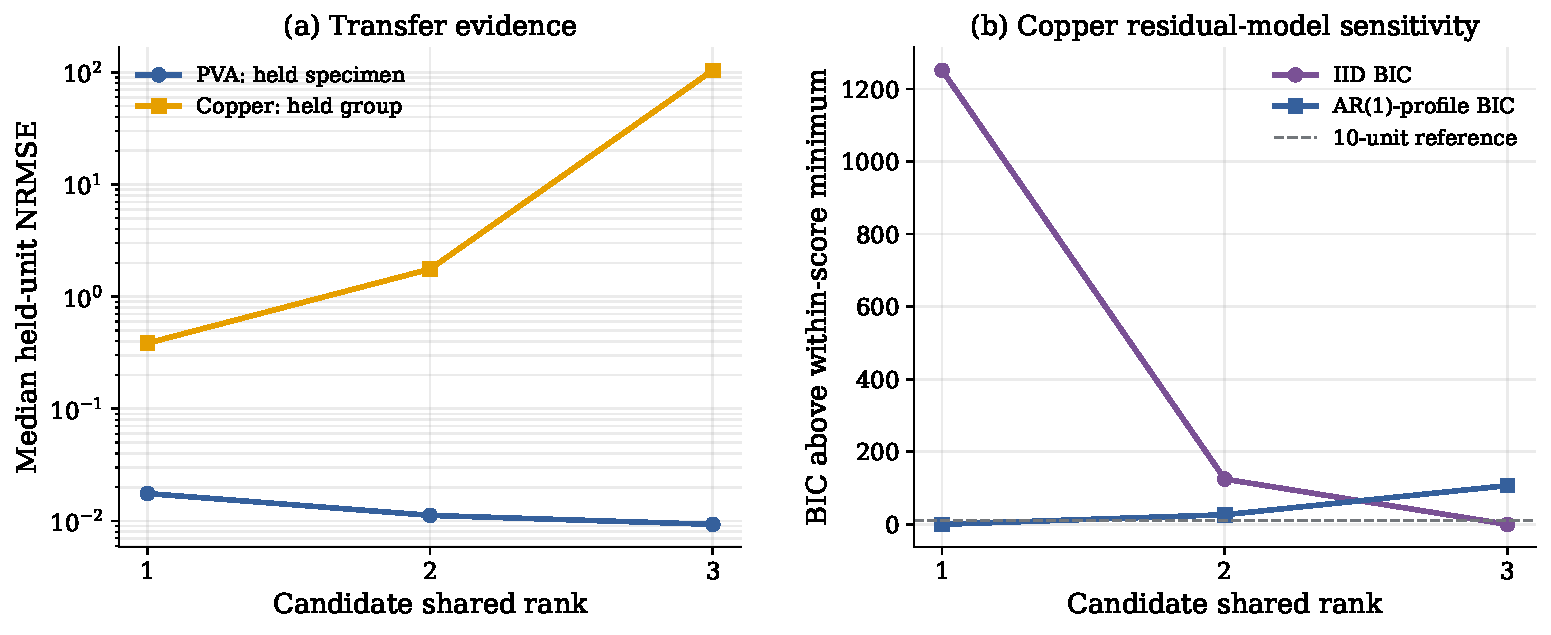
\includegraphics[width=0.98\textwidth]{fig_amm_material_evidence.pdf}
\caption{Material-relaxation evidence. (a) Held-unit errors decrease with rank for PVA but deteriorate sharply for copper-alloy material groups. (b) Copper order preference reverses after profiling an AR(1) residual model. BIC differences are shown relative to the minimum within each residual model and therefore should not be compared across the two curves as absolute likelihood values.}
\label{fig:amm-material}
\end{figure}

\subsection{Gas-sensor prediction with unresolved order}
The shared rank-three model is predictively competitive on the gas-sensor recovery task (Table~\ref{tab:gas}). It improves the median experiment error by 26.6\% relative to independent nonlinear fitting ($p=0.00110$), 80.6\% relative to fixed-grid NNLS ($p<10^{-12}$), and 8.25\% relative to Prony recurrence ($p=0.00928$).

\begin{table}[H]
\centering
\caption{Held-experiment prediction on 50 non-air gas exposures.}
\label{tab:gas}
\begin{tabular}{lcc}
\toprule
Method & Median NRMSE & Interquartile range\\
\midrule
Shared rank 3 & 0.05392 & [0.03420, 0.07168]\\
Independent nonlinear rank 3 & 0.05910 & [0.05189, 0.07471]\\
Fixed-grid NNLS & 0.25676 & [0.20728, 0.31036]\\
Prony recurrence & 0.05961 & [0.03894, 0.08373]\\
\bottomrule
\end{tabular}
\end{table}

Nevertheless, two fitted rank-three rates coalesce near $0.03765$, violating Eq.~\eqref{eq:separation}. The selection rule therefore leaves the order \indet{}. Rank three versus rank one yields a median experiment-level prediction improvement of 65.9\%, with a clustered-bootstrap 95\% interval of [58.5\%, 68.2\%], yet this predictive gain does not repair spectral non-identifiability. All 27 threshold combinations remain \indet{}, and 2/4/8-start fits return the same objective and rates.

\begin{figure}[H]
\centering
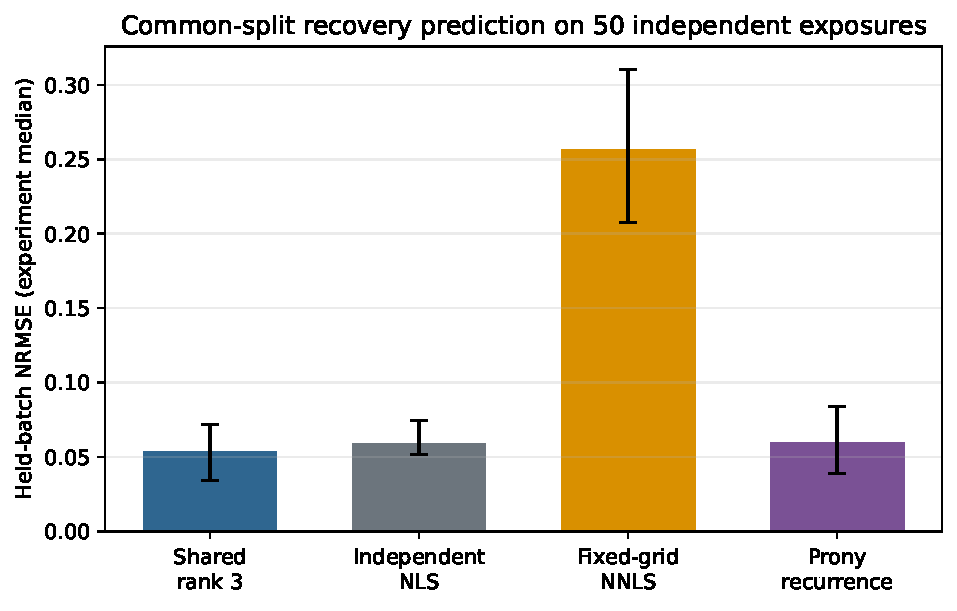
\includegraphics[width=0.94\textwidth]{fig_stage63_external_baselines.pdf}
\caption{Matched external baselines on the gas-sensor task. Points are independent exposure experiments; sensor channels are not counted as independent replicates.}
\label{fig:baselines}
\end{figure}

\begin{figure}[H]
\centering
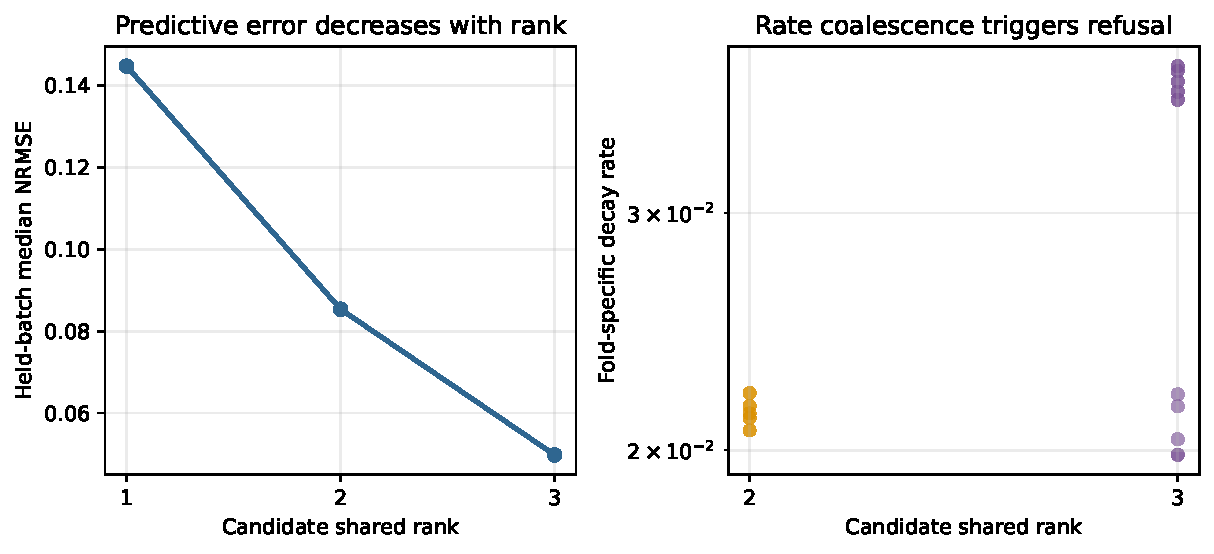
\includegraphics[width=0.94\textwidth]{fig_stage63_rank_refusal.pdf}
\caption{Predictive improvement with unresolved model order. The shared rank-three fit predicts well, but the rate-separation criterion does not support a three-timescale mechanism claim.}
\label{fig:refusal}
\end{figure}

\subsection{Hydraulic-state transfer exposes a second unresolved-order mode}
On the hydraulic task, rank two improves mean BIC from $-8509.645$ to $-9167.872$, but median held-cycle NRMSE worsens from 0.23780 to 0.51128. The median rank-two relative improvement is therefore $-73.5\%$ across 30 independent cycles (cluster-bootstrap 95\% interval $[-144.0\%,-38.4\%]$). Its fitted rates collapse at the lower bound and its local boundary index is 0.0571. Rank three also fails: held-cycle NRMSE is 0.42922, all three full-data rates coalesce near 0.069, and the boundary index is $1.85\times10^{-7}$. The decision is \indet{} for all 27 threshold combinations. Correlation sensitivity strengthens rather than reverses the unresolved-order conclusion: ordinary BIC favors rank two, whereas AR(1)-profile BIC is lowest for rank one ($-10208.35$, compared with $-9936.23$ for rank two and $-9532.14$ for rank three). The corresponding mean residual AR(1) estimates decrease from 0.68 to 0.49 and 0.40.

 For the three gas baselines, Holm-adjusted one-sided paired values are $2.66\times10^{-15}$ (fixed-grid NNLS), 0.00220 (independent nonlinear rank three), and 0.00928 (Prony); the matched predictive conclusions therefore survive within-task multiplicity correction.

The gas and hydraulic outcomes fail different criteria. Gas recovery shows predictive benefit without spectral separation, whereas the hydraulic task shows in-sample information improvement without held-condition transfer or separation.

Matched early-to-late model-family controls also rule out a trivial weak-baseline explanation. At the independent-cycle level, the shared rank-one model has median NRMSE 0.244, compared with 0.329 for a stretched exponential, 0.316 for AR(2), 0.491 for Prony recurrence, and 0.625 for fixed-grid NNLS. Within the four hydraulic baseline comparisons, Holm-adjusted paired Wilcoxon values are $7.98\times10^{-4}$ for the stretched exponential, $6.48\times10^{-6}$ for Prony, $1.20\times10^{-5}$ for NNLS, and 0.0249 for AR(2). The AR(2) bootstrap interval for the paired median difference crosses zero, so that comparison remains mixed despite its adjusted rank-test value. These controls establish predictive competitiveness on the declared transient window, not component-level physical mechanism identification.

\begin{figure}[H]
\centering

\includegraphics[width=0.96\textwidth]{fig_stage64_hydraulic_transients.pdf}
\caption{Third-domain hydraulic audit. (a) Normalized cooling-efficiency transients across controlled cooler states; bands show interquartile ranges over independent cycles. (b) Held-cycle prediction error and the projected-sensitivity boundary diagnostic. The latter is a within-rank identifiability indicator, not a cross-rank performance score.}
\label{fig:hydraulic}
\end{figure}

\subsection{Controlled tests of the recommended extension combination}
Four controlled analyses used 12 independent seeds (Fig.~\ref{fig:extensions}). For damped oscillations, replacing three positive real poles with one stable conjugate pair reduced median held-horizon NRMSE from 0.12102 to 0.002079, a 98.3\% relative reduction (one-sided paired Wilcoxon $p=2.44\times10^{-4}$), and recovered damping 0.16 and frequency 2.2 within numerical tolerance. Under declared group drift, partial pooling reduced median NRMSE from 0.04806 to 0.004249 (91.2\%; $p=2.44\times10^{-4}$). On dense log-normal relaxation spectra, a 32-point nonnegative grid improved over a rank-three finite fit by a median 59.3\%; the predeclared 20\% mismatch threshold left the finite-mechanism order unresolved in 11 of 12 seeds. This comparison diagnoses finite-model-class inadequacy; it does not identify the generating spectrum. With 39 independent calibration groups, the group-conformal analysis produced a 5.0\% mean false-alarm rate on exchangeable controls and 100\% empirical detection on the constructed shifted alternative. The latter is a power observation, whereas the coverage statement applies only to the exchangeable control design.

\begin{figure}[H]
\centering
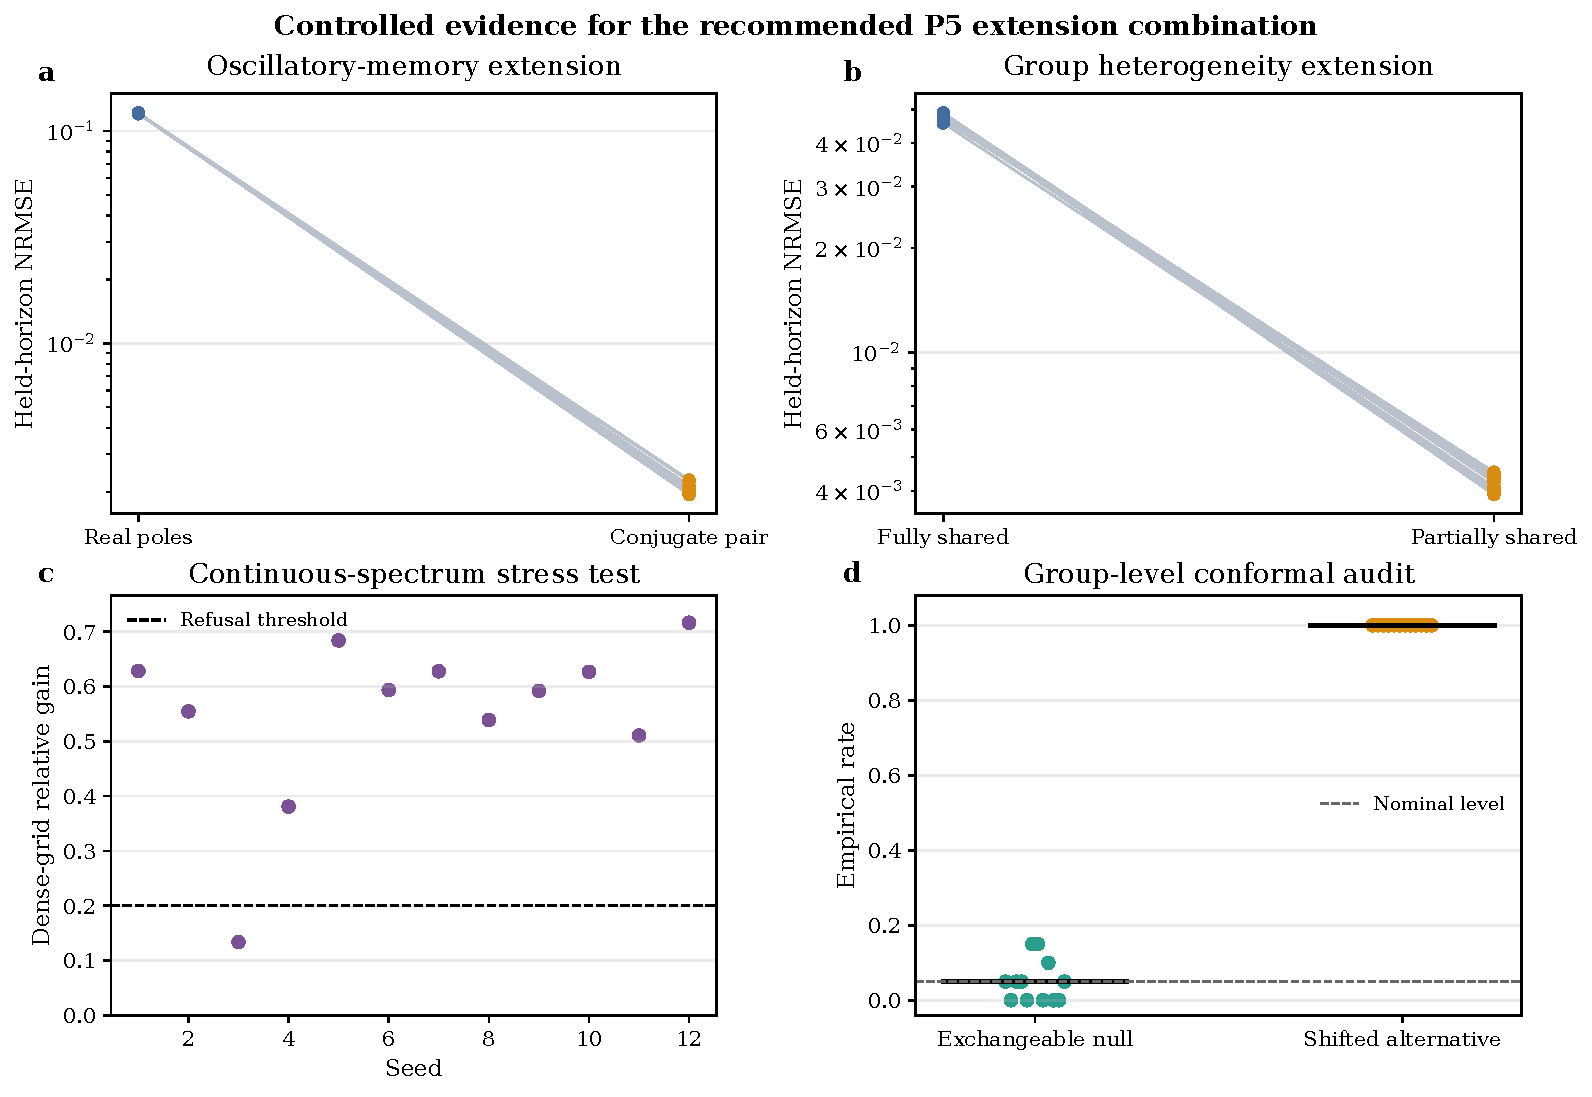
\includegraphics[width=0.96\textwidth]{fig_stage66_extension_combination.pdf}
\caption{Controlled extension analyses. (a) Positive-real-pole and conjugate-pair extrapolation on damped oscillations. (b) Fully shared and partially shared rates under group heterogeneity. (c) Dense-spectrum gain over a rank-three finite model; the dashed line is the declared mismatch threshold. (d) Group-level conformal false-alarm and shifted-alternative detection rates. Panels compare only methods within the same controlled task.}
\label{fig:extensions}
\end{figure}
\section{Discussion and modelling implications}
The experiments establish a distinction between approximation quality and mechanism support. On PVA, cross-specimen prediction, information gain, rate stability, and separation agree at the full observation horizon. On the copper-alloy task, held-material prediction and residual-aware model selection support a shared rank-one empirical state, while ordinary BIC alone would over-rank the response. On the gas task, prediction favors a richer model but separation rejects its mechanistic interpretation. On the hydraulic task, BIC favors extra modes while transfer and separation reject them. A workflow that reports only the best in-sample or predictive rank would erase these different outcomes.

The nonmonotone PVA boundary also cautions against equating longer records or denser grids with monotonically stronger evidence. Additional tail coverage can expose a slow mode, but correlated residuals reduce effective information and an enlarged rate range can worsen conditioning. The boundary-factor audit is explanatory rather than causal; its purpose is to identify which assumptions should be tested before interpreting a rank transition.

In the criterion-ablation analysis, every criterion prevents an unsupported order increase on at least one fixed stress record. This diagnostic does not quantify criterion importance in an unseen population. The method is also narrower than a general memory-kernel learner: it assumes a declared common time grid, positive real rates, finite sums of decays, and grouped experimental units. Signed curve-specific amplitudes allow channel reversals but may also create cancellation. A nonnegative-amplitude semi-synthetic analysis leaves the separated-support and coalesced-unresolved findings unchanged, although equivalence on arbitrary data does not follow. The public-data results do not cover irregular grids or nonlinear state-dependent memory. Controlled extensions demonstrate numerical feasibility for stable conjugate-pole blocks and partially shared positive rates, and produce an unresolved-order outcome under a dense relaxation spectrum. They do not establish real-data identifiability or universal calibration for these broader classes. In higher-dimensional operator settings, repeated matrix-function actions and independent reference construction replace scalar nonlinear fitting as the main costs. Extension to such settings requires an explicit reference-error budget and groupwise validation.

An order should remain unresolved when adjacent rates fall below the design-calibrated resolution, residual correlation changes the information-criterion ordering, or held-unit prediction deteriorates despite lower in-sample error. Strong nonnormality and weak latent-parameter identifiability can amplify these effects in higher-dimensional auxiliary-state models. In finite-element, mesh-free, or nonlinear PDE settings, independent references and grouped holdouts are likely to dominate the validation cost. Reference-solver accuracy and this additional cost would need to be reported explicitly.

A supported finite realization provides a compact predictive state model but does not by itself establish distinct microscopic processes. Likewise, \indet{} does not exclude a multiple-timescale mechanism; it indicates that the declared observations do not resolve one under the predeclared criteria.

\section{Reproducibility of the numerical study}
For reproducibility, the implementation package \texttt{p5\_memory\_protocol} exposes four public operations: \texttt{fit}, \texttt{evaluate}, \texttt{decide}, and \texttt{report}. Versioned JSON records store the declared domain, grouping unit, thresholds, diagnostics, decision, and scope limits. The command
\begin{verbatim}
python -m p5_memory_protocol reproduce --task uci-gas
\end{verbatim}
replays the public gas task. At manuscript assembly, 151 unit tests passed and 76 machine-readable result files parsed successfully. These checks establish internal reproducibility; independent external reproduction remains a separate requirement.

\section{Conclusion}
An identifiability-aware selection rule was evaluated for shared finite-memory models fitted to sparse grouped relaxation data. An additional mode is retained only when information gain, transfer to held units, rate stability, and timescale separation agree. The adjacent-rate bound relates this requirement to sensitivity coalescence, and the observation-design map shows that resolution is not determined by sample count alone. PVA relaxation supports a rank-three empirical realization only for the complete declared experiment. Copper-alloy relaxation supports rank one after residual correlation and held-material transfer are taken into account. In the gas and hydraulic tasks, predictive improvement coexists with unresolved model order. Depending on these diagnostics, the reported result is either a supported finite realization or insufficient resolution to assign an order. Irregular sampling, nonlinear memory, and spatially distributed material models require reference constructions beyond the setting examined here.

\section*{Data and code availability}
The public source datasets are identified by DOI in the references. Derived results, model-selection definitions, tests, and figure-generation scripts are stored in the project directory. The AMM-specific figures are generated from the machine-readable public-task and baseline records by \texttt{build\_amm\_evidence.py}. A repository URL and archival software DOI will be inserted only after a frozen public release has been verified.

\section*{CRediT authorship contribution statement}
\textbf{Haitao Duan:} Conceptualization, Methodology, Software, Formal analysis, Investigation, Validation, Writing--original draft, Writing--review and editing. \textbf{Ning Hu:} Conceptualization, Methodology, Supervision, Data curation, Validation, Visualization, Writing--review and editing. \textbf{Shuqun Li:} Investigation, Validation, Formal analysis, Writing--review and editing. \textbf{Chuyang Hu:} Investigation, Validation, Software verification, Writing--review and editing.

\section*{Funding}
This work was supported by the State Key Laboratory of Ocean Engineering, Shanghai Jiao Tong University (Grant No. GKZD010089), and the State Key Laboratory of Acoustics, Chinese Academy of Sciences (Grant No. SKLA202406). The funders had no role in the study design; collection, analysis, and interpretation of data; writing of the manuscript; or decision to submit the article for publication.

\section*{Declaration of competing interest}
The authors declare that they have no known competing financial interests or personal relationships that could have appeared to influence the work reported in this paper.

\section*{Declaration of generative AI and AI-assisted technologies}
During manuscript preparation, the authors used AI-assisted tools for language editing, document organization, and consistency checks. The authors reviewed and verified the resulting text, numerical claims, code outputs, and references and take full responsibility for the manuscript.

\section*{Ethics statement}
This study uses public non-human datasets and synthetic numerical experiments. No human participants, identifiable personal data, or animal experiments were involved.

\section*{Author identifiers}
Haitao Duan: ORCID 0009-0006-4611-8639; Ning Hu: ORCID 0000-0002-2718-0385; Shuqun Li: ORCID 0009-0007-1787-685X; Chuyang Hu: ORCID 0009-0007-9255-018X.

\bibliographystyle{unsrt}
\bibliography{references}
\end{document}






